\section*{Dati e risultati}

\subsection*{Circuito invertente}

Il primo circuito studiato sfrutta l'opamp LM741 al fine di amplificare e sfasare di $180^\circ$ il segnale in ingresso ($V\ped{in}$). Il circuito che abbiamo realizzato è illustrato in Figura \ref{fig:amp_inv}.
Questo circuito è alimentato con una tensione costante positiva di $\SI{+15}{\volt}$ e una negativa di $\SI{-15}{\volt}$.
Abbiamo collegato in ingresso un segnale sinusoidale ($V\ped{in}$) ottenuto grazie al generatore di onde.

Dal momento che vogliamo che tale circuito abbia un guadagno ($G$) di circa 10 dobbiamo dimensionarlo. In particolare, facendo l'analisi circuitale si ottiene che vale la relazione:

\begin{equation}
        G\,=\,-\frac{V\ped{out}}{V\ped{in}}\,=\,-\frac{R_2}{R_1} \qquad \implies \qquad |R_2|\,=\,10\,|R_1|
        \label{eq:g}
\end{equation}
%
dove $R_1$ e $R_2$ sono le resistenze riportate in figura, $V\ped{in}$ il segnale in ingresso e $V\ped{out}$ il segnale in uscita. Quindi, per non avere correnti troppo elevate all'interno del circuito (che dissiperebbero energia), abbiamo deciso di porre $R_2\,=\,\SI{100}{\kilo\ohm}$ e $R_1\,=\,\SI{10}{\kilo\ohm}$.

È stato quindi verificato che il guadagno di tale circuito, a frequenza fissta $\nu\,=\,\SI{1}{\kilo\hertz}$, fosse costante. A tal fine abbiamo misurato $V\ped{out}$ al variare dell'ampiezza del segnale in ingresso $V\ped{in}$. Poichè il guadagno è circa costante al variare dell'ampiezza, sfruttando la relazione (\ref{eq:g}) abbiamo fatto la media dei valori di $G$ così ricavati e abbiamo ottenuto che il guadagno del nostro circuito vale:

\begin{equation}
        G\,=\, 9.80 \pm 0.05
\end{equation}

Successivamente abbiamo deciso di studiare come varia il guadagno al variare della frequenza di $V\ped{in}$, mantenendo costante l'ampiezza $V\ped{in}$ a 515 mV picco-picco. Quello che abbiamo ottenuto è riportato in Figura \ref{fig:g_vs_freq}.

\begin{SCfigure}
    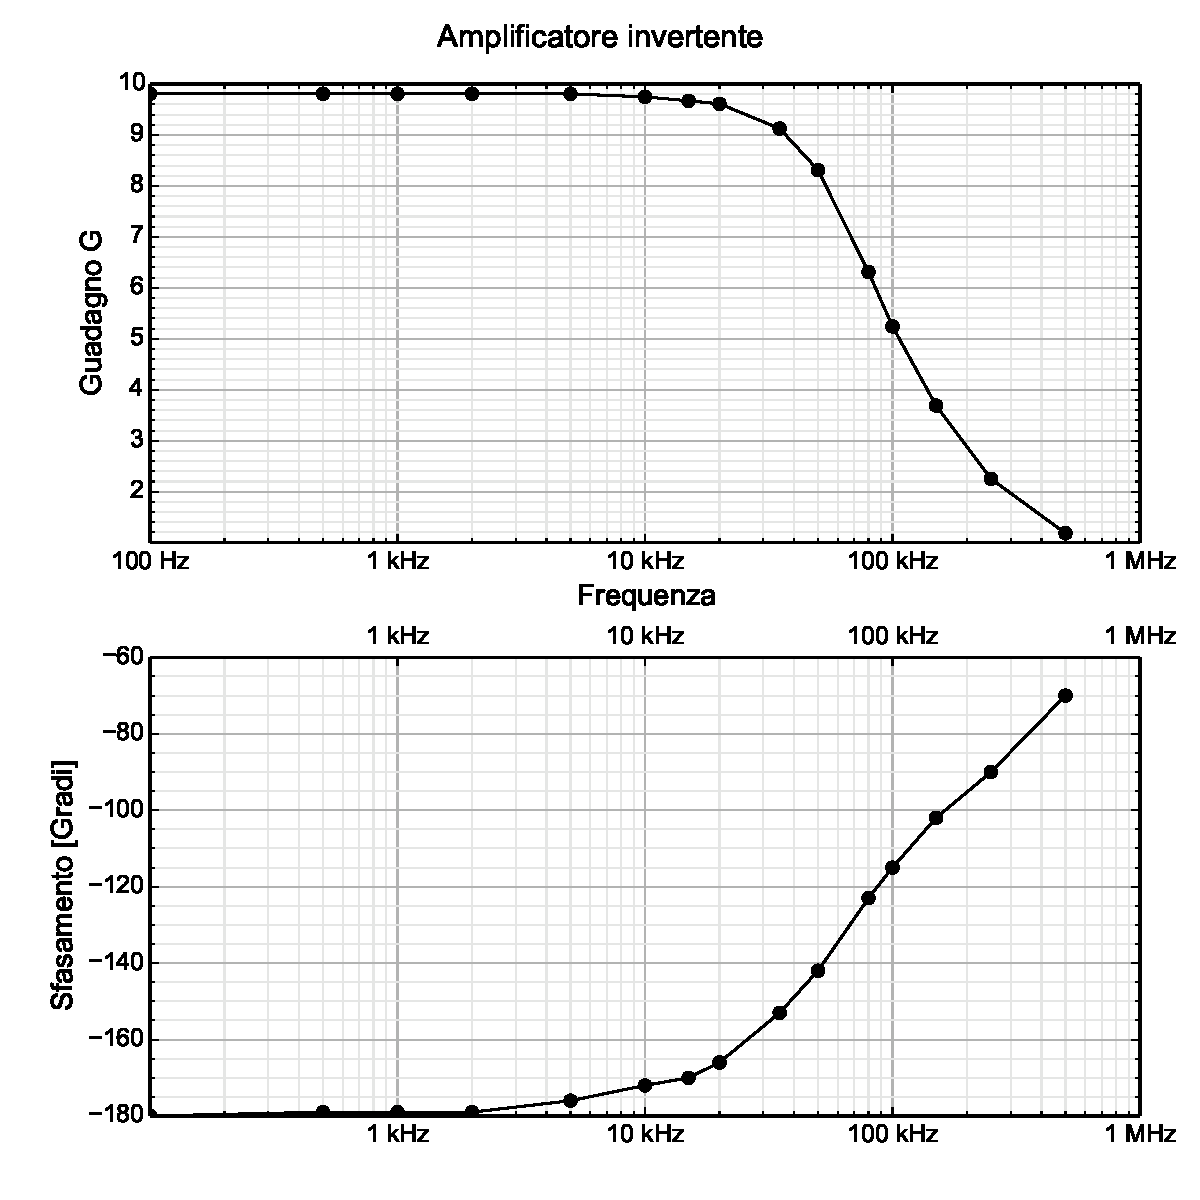
\includegraphics[width=0.75\textwidth]{amp_inv.pdf}
    \caption{La figura mostra gli andamenti di guadagno e sfasamento in funzione della
        frequenza dell'onda sinusoidale in ingresso per il circuito \ref{fig:amp_inv}. L'ampiezza del segnale è
        stata mantenuta costante a 515 mV picco-picco. Le barre d'errore non sono riportate percè simili alla dimensione
        dei punti. Tra i 10 kHz e i 20 kHz il segnale il circuito inizia a tagliare. Il punto -3dB è a circa a 100 kHz.
        Inoltre il circuito sfasa anche l'uscita e lo sfasamento varia con la frequenza, anche se non è proprio di 90$^\circ$
        a 100 kHz, ma circa 110$^\circ$. Il circuito si comporta come un filtro passa-basso ed è quindi adatto ad essere usato
        per basse frequenze.}
    \label{fig:g_vs_freq}
\end{SCfigure}

Infine abbiamo trovato i valori di ampiezza del segnale in uscita $V\ped{out}$, a frequenza costante $\nu\,=\,\SI{1}{\kilo\hertz}$ di $V\ped{in}$, per i quali si verifica il fenomeno del clamping. Tali valori sono risultati essere:

\begin{equation}
        V\ped{out}^{+}\,\simeq\,\SI{14.2}{\volt} \qquad \text{e} \qquad V\ped{out}^{-}\,\simeq\,\SI{-13.1}{\volt}
        \label{eq:clamping_1}
\end{equation}

\subsection*{Circuito non invertente}

Questo circuito, come il precedente, sfrutta l'op-amp LM741 al fine di ottenere un'amplificazione del segnale in ingresso $V\ped{in}$, ma in questo caso non è presente uno sfasamento di $180^\circ$ tra i due segnali ($V\ped{in}$ e $V\ped{out}$).
Il circuito utilizzato è riportato in Figura \ref{fig:amp_noninv}. Le sue specifiche sono esattamente uguali a quelle del circuito descritto in precedenza a parte il fatto che le due resistenze $R_1$ e $R_2$ sono posizionate in punti differenti del circuito.

Anche in questo caso abbiamo svolto delle misure di $V\ped{out}$ in funzione di $V\ped{in}$, mantenedo costante la frequenza $\nu\,=\,\SI{1}{\kilo\hertz}$ di $V\ped{in}$. Dall'analisi del circuito risulta che 

\begin{equation}
    G \,=\, 1 + \frac{R_2}{R_1} = 10.66 \pm 0.06
\end{equation}
%
dove il valore numerico è la media dei valori che abbiamo ottenuto per diverse ampiezze di $V\ped{in}$.

Successivamente abbiamo valutato l'andamento di $V\ped{out}$ in funzione della frequenza di $V\ped{in}$, tenendo fissa
l'ampiezza del segnale in ingresso a 519 mV, e abbiamo ottenuto quanto illustrato in Figura \ref{fig:g2}.

\begin{SCfigure}
    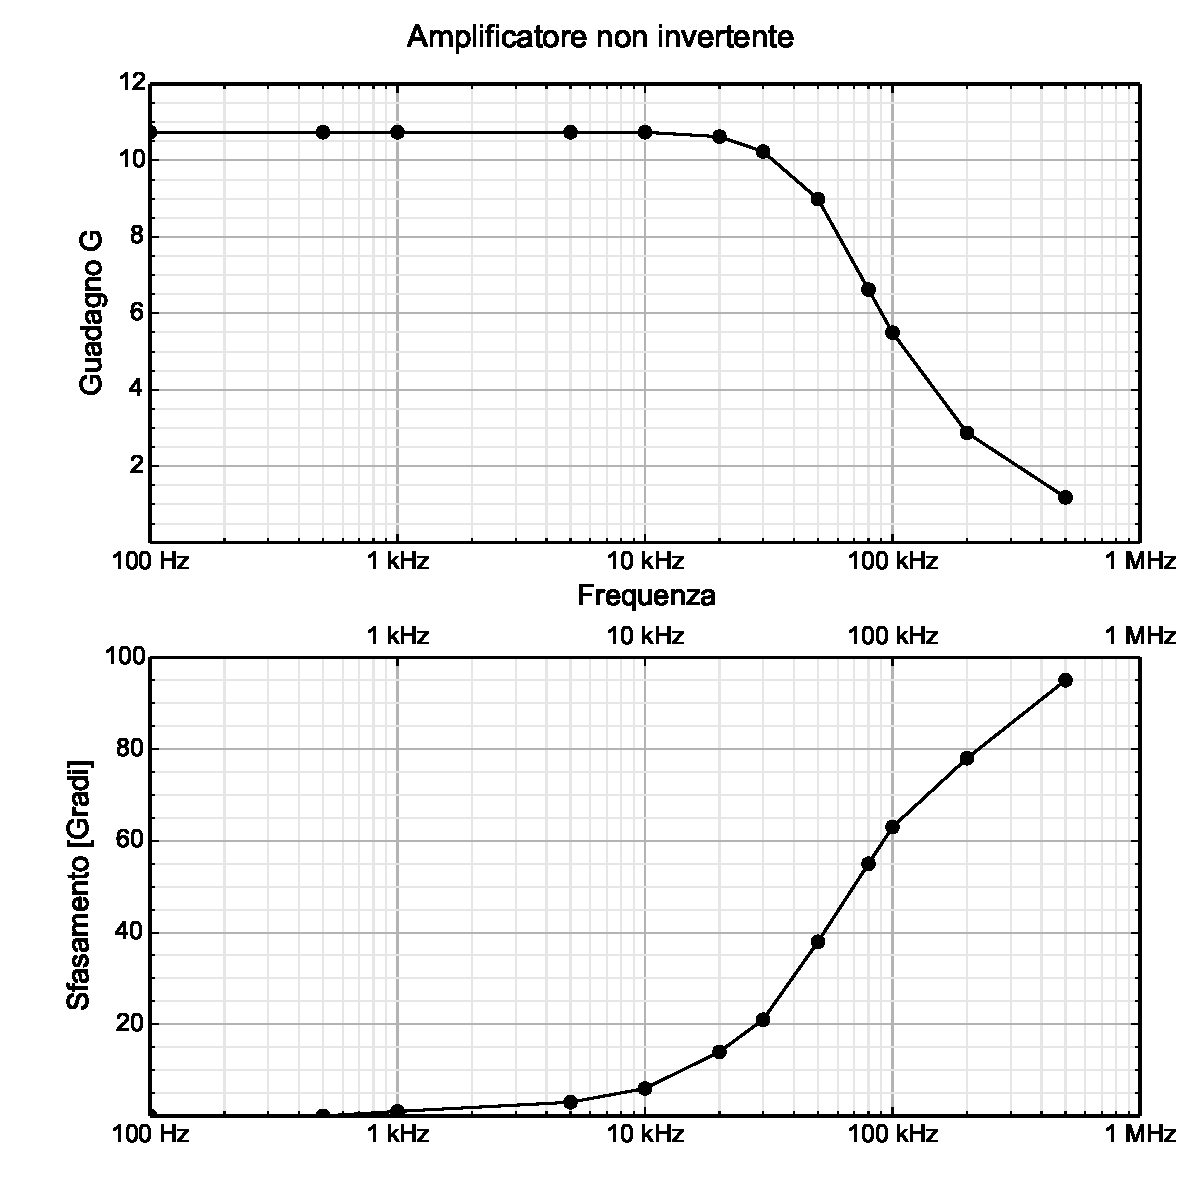
\includegraphics[width=0.75\textwidth]{amp_ninv.pdf}
    \caption{La figura mostra gli andamenti di guadagno e sfasamento in funzione della
        frequenza dell'onda sinusoidale in ingresso per il circuito \ref{fig:amp_ninv}. L'ampiezza del segnale è
        stata mantenuta costante a 519 mV picco-picco. Le barre d'errore non sono riportate percè simili alla dimensione
        dei punti. Anche in questo caso il circuito si comporta come un passa basso, con frequenza di taglio
        (-3dB) a circa a 100 kHz. La degradazione del guadagno comincia tra i 20 kHz e i 30 kHz.
        Lo sfasamento varia con la frequenza e a 100 kHz è di circa 65$^\circ$.}
    \label{fig:g2}
\end{SCfigure}

Infine, come nell'analisi dl circuito precedente, abbiamo trovato i valori di ampiezza del segnale in uscita $V\ped{out}$, a frequenza costante $\nu\,=\,\SI{1}{\kilo\hertz}$ di $V\ped{in}$, per i quali si verifica il fenomeno del clamping. Tali valori sono risultati essere:

\begin{equation}
        V\ped{out}^+\,\simeq\,\SI{13.2}{\volt} \qquad \text{e} \qquad V\ped{out}^-\,\simeq\,\SI{-13.1}{\volt}
\end{equation}

\subsection*{Circuito sommatore}

Come passo successivo abbiamo utilizzato il nostro amplificatore operazionale per realizzare un circuito sommatore, rappresentato in Figura \ref{fig:sum}. Questo circuito ha lo scopo di ricevere in ingresso più segnali $V_i$ e di restituire in output la loro somma pesata sui relativi valori di $R_i$. In formule:

\begin{equation}
        V\ped{out}\,=\,\sum_{i=1}^{n}{\frac{R}{R_i} \cdot V_i}
\end{equation}
%
dove $R$ è il valore di resistenza della retroazione, $V_i$ sono i vari valori di tensione in ingresso e $R_i$ i valori di resistenze dell'input corrispondente.

Come è facile notare, nel nostro caso, ci sono solo due valori di $V_i$ ovvero $V_1$ e $V_2$ e $R_1$, $R_2$ ed $R$ hanno lo stesso valore di $\SI{10}{\kilo\ohm}$. Inoltre il segnale $V_1$ è fornito dal generatore d'onde, quindi ne potevamo variare l'ampiezza e la frequenza, mentre il segnale $V_2$ è ottenuto grazie alla sorgente di tensione alternata, di fequenza $\nu_0\,=\,\SI{50}{\hertz}$, con un'ampiezza picco-picco di $\SI{7.5}{\volt}$. Anche in questo caso l'amplificatore operazionale è alimentato tra una tensione posistiva di $\SI{+15}{\volt}$ e una negativa di $\SI{-15}{\volt}$.

Pertanto una volta montato il circuito ci siamo serviti dell'oscilloscopio per verificare che effettivamente quello che abbiamo realizzato fosse un circuito sommatore. Il risultato ottenuto è riportato in Figura \ref{fig:}

\subsection*{Circuito integratore}

In questa sezione della relazione ci occupiamo di studiare le caratteristiche del circuito illustrato in Figura \ref{fig:int} realizzato con il solito op-amp LM741.

Le specifiche del circuito sono riportate in Figura \ref{fig:int}, tuttavia facciamo notare che in ingresso ($V\ped{in}$) è stato applicato un segnale variable nel tempo sfruttando il generatore di onde.
 
Lo scopo di questo circuito, idealmente, è quello di fornire un un segnale in uscita ($V\ped{out}$) che, come dice il nome stesso, è l'integrale del segnale in ingesso ($V\ped{in}$). Ovvero matematicamente:

\begin{equation}
        V\ped{out}\,=\,-\frac{1}{R_1C} \int_{t}{V\ped{in}dt}\,+\,c
\end{equation}
%
dove $R_1$ e $C$ indichiamo rispettivamente la resistenza 1 e la capacità del circuito di feedback, $c$ è la costante di integrazione, e $V\ped{in}$ è il segnale in ingresso che è funzione del tempo.

Di questo circuito ne abbiamo verificato il corretto funzionamento acquisendo, grazie all'oscilloscopio, il segnale in uscita $V\ped{out}$ per varie forme d'onda in ingresso, generate dal generatore d'onda. I risultati ottenuti sono riportati in Figura \ref{fig:}.

\subsection*{Circuito derivatore}

Per finire abbiamo montato un circuito derivatore, illustrato in Figura \ref{fig:diff}.

Le specifiche di tale circuito sono riportate in Figura \ref{fig:diff}, tuttavia facciamo notare che in ingresso ($V\ped{in}$) è stato applicato un segnale variable nel tempo sfruttando il generatore di onde.

Lo scopo di queto circuito è quello di fornire in output un segnale ($V\ped{out}$) che è la derivata temporale del segnale in ingresso ($V\ped{in}$). In formule si dovrebbe ottenere che, se il circuito fosse ideale:

\begin{equation}
        V\ped{out}\,=\,-R_1C \cdot \frac{dV\ped{in}}{dt}
\end{equation}
%
dove con $R_1$ indichiamo la resistenza in serie al condensatore $C$ e $V\ped{in}$ è il segnale in ingresso al circuito.

Anche per questo circuito abbiamo voluto verificarne il corretto funzionamento, sfruttando l'oscilloscopio, osservando che $V\ped{out}$ sia effettivamente la derivata del segnale in ingresso $V\ped{in}$. Questo è stato fatto per varie forme d'onda in ingresso al circuito. I risultati ottenuti sono illustrati in Figura \ref{fig:}
